\documentclass[a4paper,12pt]{amsart}
\usepackage[T1, T2A]{fontenc}

\usepackage[utf8]{inputenc}

\usepackage{amsmath}
\usepackage{amsthm}
\usepackage{graphicx}
\usepackage{amssymb,stackengine}
%\usepackage[english]{babel}
\usepackage[ukrainian, english]{babel}

\usepackage{listings}
% \usepackage[colorlinks]{hyperref}
\usepackage{hyperref}
\usepackage[title]{appendix}


% template
\frenchspacing \righthyphenmin=2 \emergencystretch=5pt
\hfuzz=0.5pt \tolerance=400 \oddsidemargin 5mm \evensidemargin 5mm
\textwidth 160mm \textheight 230mm

\hoffset=-0.5cm \voffset=-1.0cm

\renewcommand\baselinestretch{1.1}



\usepackage{xcolor}

% links
\hypersetup{
	colorlinks=true,
	linkcolor=blue,
	filecolor=magenta,      
	urlcolor=cyan,
}

% coloring of listings


\definecolor{codegreen}{rgb}{0,0.7,0}
\definecolor{codegray}{rgb}{0.4,0.4,0.4}
\definecolor{codepurple}{rgb}{0.58,0,0.82}
\definecolor{backcolour}{rgb}{0.95,0.95,0.92}

\lstdefinestyle{mystyle}{
	backgroundcolor=\color{backcolour},   
	commentstyle=\color{codegray}\textit,
	keywordstyle=\color{magenta},
	numberstyle=\tiny\color{codegray},
	stringstyle=\color{codepurple},
	%	basicstyle=\ttfamily\footnotesize,
	breakatwhitespace=false,         
	breaklines=true,                 
	captionpos=b,                    
	keepspaces=true,                 
	numbers=left,                    
	numbersep=3pt,                  
	showspaces=false,                
	showstringspaces=false,
	showtabs=false,                  
	tabsize=2
}

\lstset{style=mystyle}


% path to images
\graphicspath{ {../graphs/} }
\usepackage[left=2cm,right=2cm,
    top=2cm,bottom=2cm,bindingoffset=0cm]{geometry}
\title{ 	Складність проблеми слів в Ханойських групах }
\author{ David Zashkolny }
\date{March 2020}

\newtheorem{definition}{Definition}

\newtheorem{statement}{Statement}

\newtheorem{theorem}{Theorem}
\newtheorem{lemma}[theorem]{Lemma}


\begin{document}


\thispagestyle {empty}
\begin{center}
	\large  Київський Національний Університет ім. Т.Г. Шевченка \\
	Механіко-математичний факультет \\
	Кафедра алгебри і комп'ютерної математики \par
\end{center}


\begin{center}
	\vskip0cm plus 2fill
	\vspace{2.5cm} {\bf Курсова робота}\\
	
	%{\bf на здобуття ступеня магістра математики}\\
	{\bf на тему:}\\
\end{center}


\vskip0cm plus 1.0fill



\begin{center}\bf
	{\LARGE 
		Складність проблеми слів в Ханойських групах \par}
\end{center}

\vskip0cm plus 1.5fill

\hangindent=7cm \hangafter=0 \noindent  
студента 3-го курсу\\
механіко-математичного факультету\\
{\bf Зашкольного Давида Олександровича}\\[2cm]
Керівник :\\
Доцент кафедри, доктор фiзико-математичних наук\
{\bf Бондаренко Євген Володимирович}


\vskip0cm plus 1.5fill

\vskip5cm plus 1.5fill            
\begin{center}
	КИЇВ --- 2020
\end{center}

\newpage
\pagenumbering{arabic}

%\newpage
\tableofcontents

\newpage

\section{Introduction}

This article presents investigation of algorithm for solving word problem in 
the Hanoi Tower Group. Here we show that such algorithm exists and its asymptotic growth
depends on one quality of elements called $size$. We also denote the explicit form of 
elements with the biggest possible size and exact formula to calculate it (spoiler: it will 
be $O(n \log n)$ where $n$ means a word's length). For making this to be possible we 
introduce a tree-like representation of elements, investigate its structure and some interesting 
properties, including distribution of n-th level segments. With such tool we also try to 
explain an average size of elements which is non-trivial question.


\section{Hanoi Tower Game and automaton groups}
 
Fix integers $k, n \in \mathbb{N}, k \ge 3$. The Hanoi Tower Game is played on k pegs, labeled by
$0, 1, ... k-1$, with n disks labeled by $1, 2, ... n$. All the $n$ disks have different
size and their labels mean the relative size of disks from the smallest to the biggest. 
Any placement of these $n$ disks on $k$ pegs which satisfies condition that there is no 
a bigger disk upon the smaller one is a correct \textit{configuration}. In a single step 
a gamer can move the top disk from one peg to another iff the result placement is a valid configuration. 
Thus, for any two pegs with non-zero number of disks in total there is only one possible move which 
involves these two pegs (the smaller top disk will be moved). At the beginning all the disks are placed 
on peg $0$ and the goal of the game is to move all of them to peg $1$ in the smallest possible numbers of 
steps (check \cite{HaoniDesk} for more information).

\begin{figure}[h]
	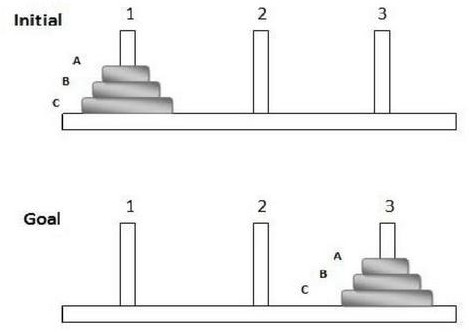
\includegraphics[scale=0.4]{../graphs/hanoi_tower.jpg}
	\centering
\end{figure}

As in the \cite{Hanoi2} we consider the free monoid $X^*$ of words over the alphabet $X = \{0,... k-1\}$.
The structure of an $X$ can be represented as a $k$-regular rooted tree $T$ (an empty word is the root, 
the $n$-th level consists of $n$-length words and for each $w \in X^*$ a corresponding vertex in the 
tree has children $w x$ for $x = 0, ... k-1$). Define recursive functions 
$a_{(ij)} : X^* \rightarrow X^*$ in such a way: 
$$ 
a_{(ij)}(iw) = jw, \quad a_{(ij)}(jw) = iw, \quad a_{(ij)}(xw) = xa_{(ij)}(w), \quad for \, x \notin \{i, j\}
$$
We can think about these functions either as moves in the Hanoi Tower Game (the word 
$(w = x_1 x_2... x_n) \in X^*$ represents a valid configuration of $n$ disks on $k$ pegs) 
or as automorphisms of the $T$. Since any automorphism $g$ of $T$ can be (uniquely)
decomposed as $\pi_g (g_0, g_1, ... g_{k-1})$ (where $\pi_g \in S_{k}$ is called 
\textit{root permutation} of $g$ and $g_x, \, x = 0, ... k-1$, are the tree automorphisms 
called the (first level) $sections$ of $g$), defined functions also have such representation:
$$
a_{(ij)} = (i j) (a_0, a_1, ... a_{k-1}),
$$ 
where $a_s$ is the identity function (automorphism) if $s \in \{i, j\}$ and $a_s = a_{(ij)}$ otherwise.
\\

\begin{definition}
\textit{Hanoi Towers group on k pegs}, $k \ge 3$, is the group 
$H^{(k)} = \left\langle \left\{ a_{(ij)} | 0 \le i < j \le k - 1 \right\}\right\rangle$.
\end{definition}

Note: $H^{(k)}$ is an example of \textit{automaton groups} (see \cite{Auto}).

\begin{figure}[h]
	\centering
	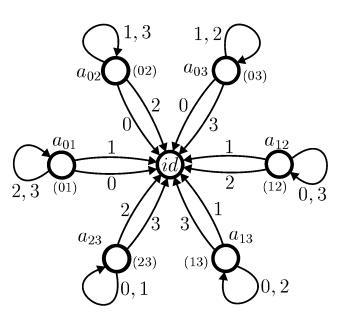
\includegraphics[scale=0.4]{../graphs/automaton_h4.jpg}
	\label{automaton}
	\caption{The automaton generating $H^{(4)}$.}	

\end{figure}


\section{Word problem and Trees}

Now let's take a look at the $H^{(3)}$ group. Hereafter define generators:  

$$ a := a_{(12)} = (1 2) (e, e, a_{(12)}) $$
$$ b := a_{(13)} = (1 3) (e, a_{(13)}, e) $$
$$ c := a_{(23)} = (2 3) (a_{(23)}, e, e) $$

Let's also introduce a new symbol $\delta$ which means a recursive call (its $\delta$ because 
this letter similar to $\circlearrowleft$). Thus, we
have such representation of the $H^{(3)}$ atomic elements:

$$ e = () (\delta, \delta, \delta), \quad a = (1 2) (e, e, \delta), \quad 
b = (1 3)(e, \delta, e), \quad c = (2 3)(\delta, e, e)$$

With these denotations it's easy to write simple multiplication rules for any 
$g \in H^{(3)}, \, g = \pi (g_1, g_2, g_3):\\ \quad g a = \pi * (12) (g_2, g_1, g_3a), \quad  
g b = \pi* (13) (g_3, g_2b, g_1), \quad g c = \pi * (23) (g_1c, g_3, g_2)$ (henceforth multiplication 
in $S_3$ defined in the such way: $(\pi * \sigma) (x) = \sigma(\pi(x))$).

Note that $a^2 = b^2 = c^2 = e$ (due to definition of the automorphism's action or 
it's also implies from the multiplication rules). It allows us to consider at the same 
time a free group $G$ over an alphabet $\Sigma = \{a, b, c\}$ with relations 
$aa = bb = cc = \lambda$ where $\lambda$ is an empty word. 
\textit{The word problem} is to describe an entire set of elements $R$ 
such that quotient $G / \left\langle R \right\rangle$ is isomorphic to $H^{(3)}$ 
(a.k.a presentation of the group). This problem also can be reinterpret 
as determining whether element $g \in G$ is trivial or not.
\\

It should be pointed out that in \cite{HRepr} a full presentation for $H^{(3)}$ is obtained. It is: 

$$ H^{(3)} = \left\langle 
	a, b, c,\, |\, a^2, b^2, c^2, \tau^n(w_1), \tau^n(w_2), \tau^n(w_3), \tau^n(w_4) \, \forall n \ge 0
\right\rangle $$

where $\tau$ is an endomorphism of $H^{(3)}$ defined by the substitution

$$ a \mapsto a, \quad b \mapsto b^c, \quad c \mapsto c^b$$

and where 
$$ w_1 = [b, a][b, c][c, a][a, c]^b[a, b]^c[c, b] $$
$$ w_2 = [b, c]^a[c, b][b, a][c, a][a, b][a, c]^b $$
$$ w_3 = [c, b][a, b][b, c]^a[c, b]^2[b, a][b, c]^a[b, c]^a $$
$$ w_4 = [b, c]^a[a, b]^c[b, a]^2[a, c][a, b]^c[c, a][c, b] $$

But in this research let's forget about other relations. Since we have the homomorphism 
between $G$ and $H^{(3)}$ all the multiplication rules for the described forms of elements
from $H^{(3)}$ are also fair in the $G$. 
\\

\begin{statement}
	Any element of the $G$ can be represented as a finite rooted 3-regular tree with labels.
\end{statement}

\begin{proof}
	
	Let there is any $w_g \in G$ and relative to it $g \in H^{(3)}$. Since $g = \pi (g_1, g_2, g_3)\,$ 
	$w_g$ also satisfies corresponding representation $w_g = (w_1, w_2, w_3)$ where $w_i \in G, \, i = 1..3$.
	Due to structure of the atomic elements and multiplication rules $|w_i| \le |w_g|$ and  
	$|w_i| = |w_g| \, \Leftrightarrow \, w_i = w_g, \, w_j = e, \, j = 1..3, j \ne i$. 
	Moreover, $|w_1| + |w_2| + |w_3| = |w_g|$. Thus, we can augment this representation to the next 
	levels until we get to recursive calls which we substitute with $\delta$. Hence, we have a finite 
	graph and it will have no cycles if we label each vertex as $w_{i_1 i_2 ... i_k}$ recursively:
	$$
	w_{i_1 i_2 ... i_k} = (w_{i_1 i_2 ... i_k 1},\, w_{i_1 i_2 ... i_k 2},\, w_{i_1 i_2 ... i_k 3})
	$$
	
	
	
\end{proof}


\begin{figure}[h]
	\centering
	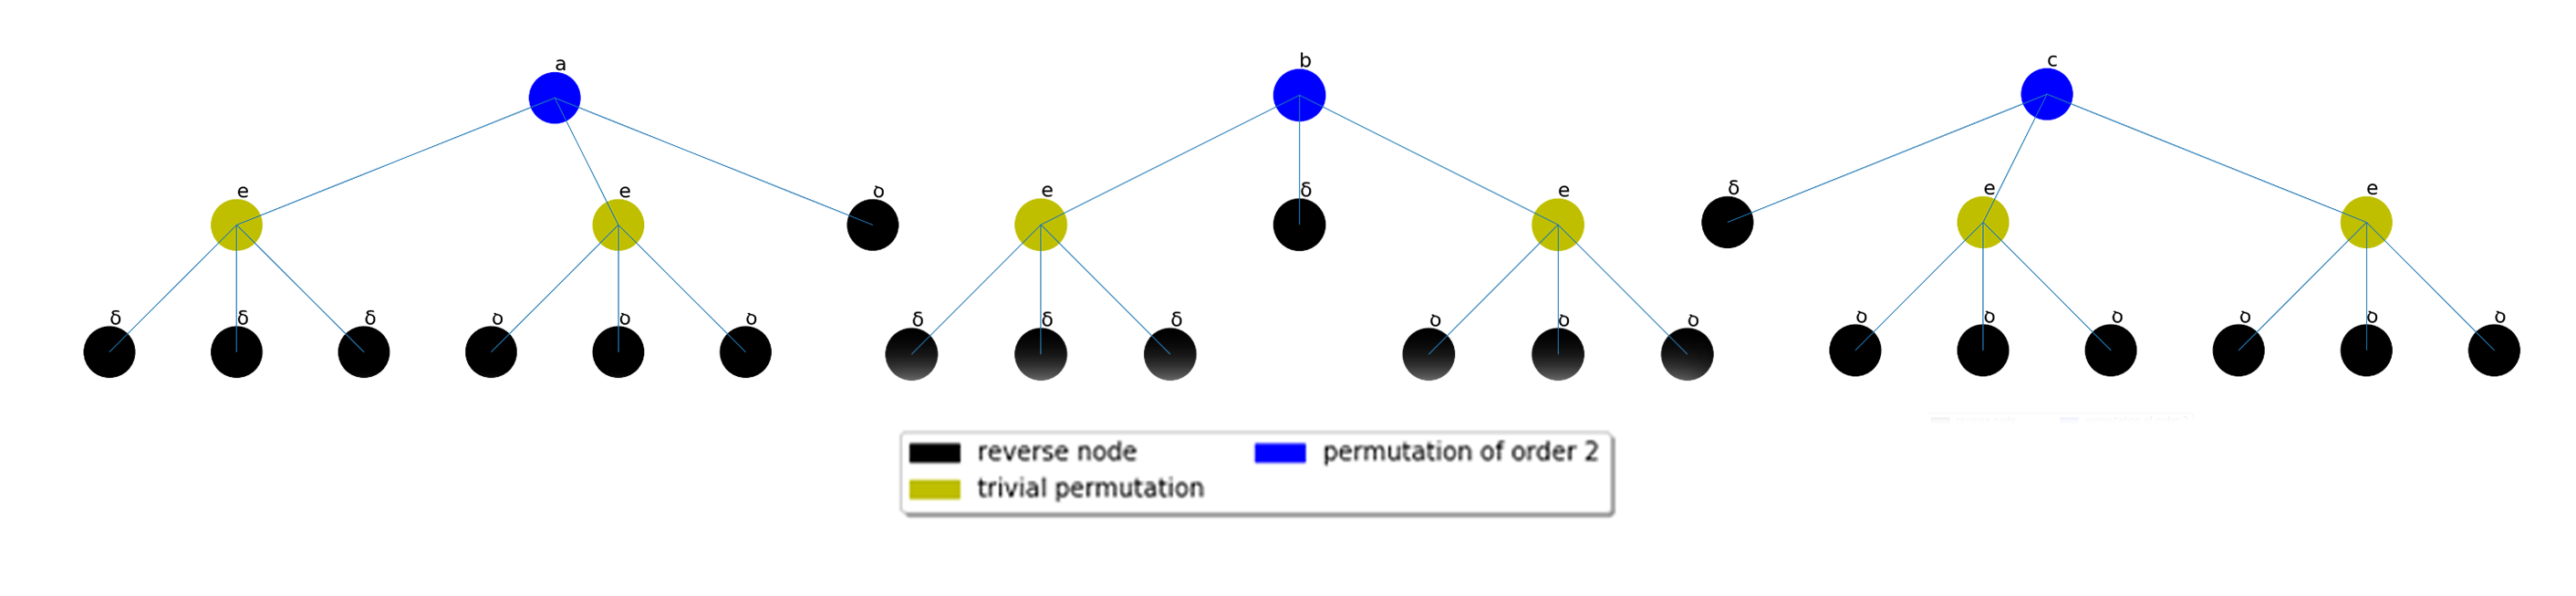
\includegraphics[scale=0.13]{../graphs/a_b_c.png}
	\caption{Corresponding trees for atomic elements.}
	\label{a_b_c}	
\end{figure}

Hereupon for $w \in G$ we define its tree as $T_w$.

Now we can define functions $v(w)$ which means amount of vertices in the $T_w$ and 
$h(w)$ which means height of the $T_w$ (in both cases excluding $\delta$ vertices).

\theoremstyle{definition}
\begin{definition}
	Function $\textbf{size} : G \rightarrow \mathbf{N} \cup \{0\}$ is defined recursively:
	
	\begin{equation}
	\label{size} 
	size(w = \pi (w_1, w_2, w_3)) =
	\begin{cases}
	0, \quad  w = e \\
	0, \quad  w = \delta  \\
	|w| + size(w_1) + size(w_2) + size(w_3)\text{,} \quad \text{otherwise}
	\end{cases}
	\end{equation}
\end{definition}



Thus, $size(a) = size(b) = size(c) = 1$ by definition (Fig \ref{a_b_c}).

Similarly, $size(aa) = size(bb) = size(cc) = 2, \quad size(ab) = size(ac) = ... = size(bc) = 4$

\begin{figure}[h]
	\centering
	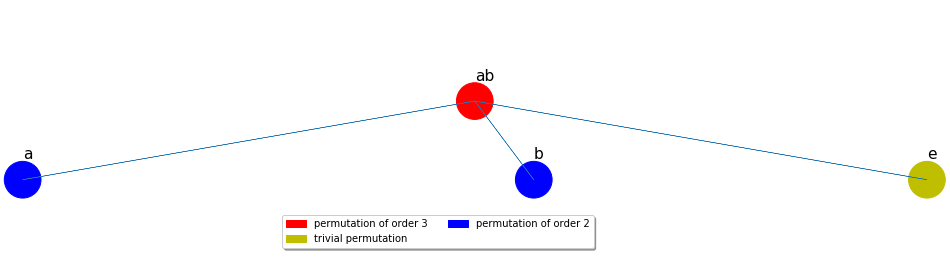
\includegraphics[scale=0.3]{../graphs/ab.png}
	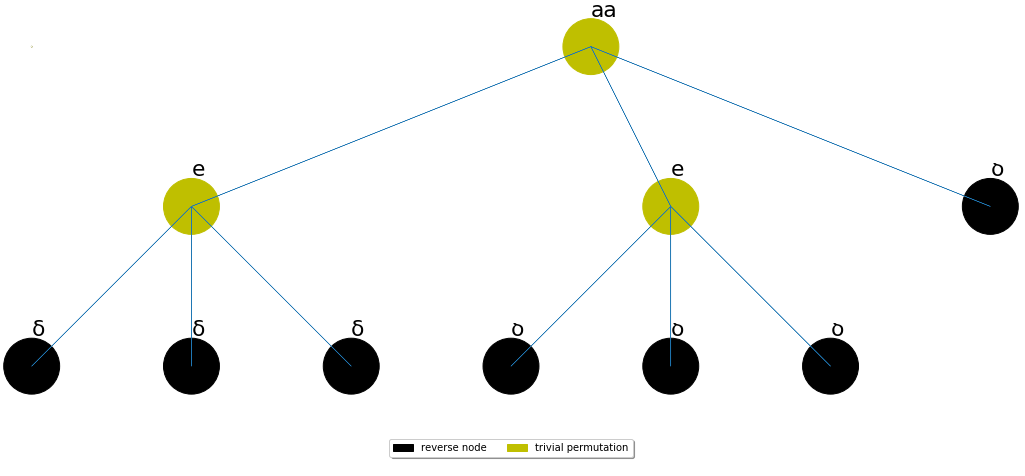
\includegraphics[scale=0.23]{../graphs/aa.png}
	\caption{The words from $\{a, b, c\}^2$ can be divided into 2 classes.}
	\label{second_order}
\end{figure}


\section{Algorithm description}

Instead of describing explicit form of the trivial elements we consider an algorithm 
for checking whether given element $w \in G$ is trivial or not in guaranteed time  
$O(n \log{n})$ where $n = |w|$. Also we will try to investigate an average case which is 
the main goal of this article. 
\\ 

Fix $w = (w_1, w_2, w_3) \in G$ and a homomorphism $\varphi : G \rightarrow H^{(3)}$ such that 
$\varphi(w_a) = a, \, \varphi(w_b) = b, \, \varphi(w_c) = c, \, \varphi(\lambda) = e$. 

\newpage

Recursive conditions of triviality for $\varphi(w)$ are pretty simple: 

\begin{itemize}
	\item The root permutation of $\varphi(w)$ should be an identity one
	\item $\forall \, i = 1 ... 3 \quad \varphi(w_i)$ is trivial  or $w_i = \delta$  
\end{itemize}

The main problem since we have a tree representation $T_w$ is to calculate the root permutation
for each vertex in the tree. 


Therefore, now we can write a full algorithm. Here is a Python-like pseudocode (well, actually 
it's real Python code, interface of used classes you can find in the appendix of this article, 
full implementation you can find at \href{https://github.com/davendiy/automata-groups}{github.com/davendiy/automata-groups})


\begin{lstlisting}[language=Python]

def is_trivial(w: AutomataGroupElement):
   
    if w.permutation != TRIVIAL_PERMUTATION:
        return False
    
    res = True
 
    # traverse all the children to make a recursive call for 
    # each w_i that isn't \lambda 
    for w_i in w.children:

        if w_i.reverse: 
            continue
        if not is_trivial(w_i):
            res = False
            break
            
    return res

\end{lstlisting}


\section{Asymptotic growth}

Let $t(w)$ determines amount of elementary operations that requires aforementioned function $is\_trivial(w)$.


\begin{statement}
	$t(w) = O(size(w))$.
\end{statement}

\begin{proof}
	For each vertex $v_s \in T_w$ that represents $s \in G$ we can compute the root permutation of $\varphi(s)$ and its
	first-level sections doing $O(|s|)$ operations. Thus,
	$$
	t(w) = \sum_{v_s \in T_w} O(|s|) = O(size(w)),\, \text{by definition (\ref{size})}.
	$$
	
\end{proof}

Therefore we can describe asymptotic growth of the function $size(w)$ and its dependence of $|w|$ will 
also give us a nice above limitation for asymptotic growth of $is\_trivial(w)$.

\section{Size. The worst case}


\begin{definition}
	\textbf{abc-subset} $X \subset  G$ is such subset: 
	
	\begin{equation}
	X = \left\{ (a^\pi b^\pi c^\pi)^k, \, (a^\pi b^\pi c^\pi)^k a^\pi, \, (a^\pi b^\pi c^\pi)^k a^\pi b^\pi  |\, k \in \mathbf{N}\cup\{0\}, \, \pi \in S_3   \right\}
	\end{equation}
	where $a^\pi$ means $S_3$ group action the alphabet $\{a, b, c\}$; \\
	$(w_1 w_2 w_3)^k$ means repeating $k$ times of the word in the parenthesis.
	\\
	
\end{definition}

\begin{lemma}
	$\forall w \in X \, w$ will have one of the next possible structures:
	$$\pi (w_1, w_2, e), \quad \pi(w_1, e, w_2), \quad \pi(e, w_1, w_2), $$
	where $w_1, w_2 \in X, \quad |w_1|, |w_2| \in
	\left\{
		\left\lfloor
			\frac{n}{2}
		\right\rfloor,
		\left\lceil
			\frac{n}{2}
		\right\rceil
	\right\}, \quad |w_1| + |w_2| = n, \quad n = |w|$
	\\
\end{lemma}

\begin{proof}
	Follows from definition of multiplication.
\end{proof}

Example: 

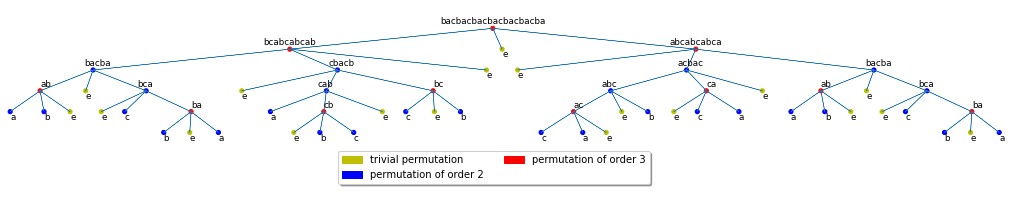
\includegraphics[scale=0.5]{../graphs/max_size_tree.png}

Therefore, here we have recursive formula for calculating function $size$ (\ref{size}) for elements from $X$:

$$size(w \in X) =: a (n) = a \left(
		\left\lfloor
			\frac{n}{2}
		\right\rfloor
	\right)
	+ a \left(
			\left\lceil
				\frac{n}{2}
			\right\rceil
		\right) + n, \quad a(1) = 1, \quad a(0) = 0, \quad n = |w|
$$

\begin{theorem}
	Exact form of function $a(n)$:
	\begin{equation}
	a(n) = \begin{cases}
	n \left(\left\lfloor \log_2 n + 1 \right\rfloor\right) + 2n - 2^{\left\lfloor\log_2 n\right\rfloor + 1}, \quad n > 0 \\
	a(0) = 0
	\end{cases}
	\end{equation}
\end{theorem}

\begin{proof}
	$$ a (n+1) = n + 1 + a \left(
		\left\lfloor 
			\frac{n+1}{2}
		\right\rfloor 	
	\right)  + a \left(
		\left\lceil 
			\frac{n+1}{2}
		\right\rceil 
	\right) = n + 1 + a \left(
		\left\lfloor 
			\frac{n}{2} 
		\right\rfloor + 1
	\right) + a \left(
		\left\lceil 
			\frac{n}{2}
		\right\rceil 
	\right)
	$$
	
	
	$$
	\text{Let} \, b(n) := a(n + 1) - a(n) = 1 + a \left(
		\left\lfloor
			\frac{n}{2}
		\right\rfloor + 1
	\right) - a \left(
		\left\lfloor
			\frac{n}{2}
		\right\rfloor
	\right) \, \text{ - auxiliary recursion.
	}	
	$$ 

	\begin{equation}
	\label{b}	
	b(n) = b\left(
		\left\lfloor
			\frac{n}{2}
		\right\rfloor
	\right) + 1, \quad b(2) = 4 \quad \Rightarrow \quad b(n) = \left\lfloor \log_2{n}\right\rfloor + 3	
	\end{equation}
	
	$$
	a (n + 1) = b(n) + b(n-1) + ... + b(1) = 
		\sum_{1 \le k \le n} \left(
			\left\lfloor
				\log_2{k} + 3
			\right\rfloor	
		\right) \quad \Rightarrow \quad a(n) = 2(n - 1) + 
		\sum_{1 \le k \le n} \left(
			\left\lfloor
				\log_2{k} + 1
			\right\rfloor	
		\right)  = 
	$$
	$$
	= \begin{bmatrix}
	   	  \text{amount of bits in all the} \\
		  \text{numbers from} \,1 \,\text{to} \,N-1
	  \end{bmatrix} = 2(n-1) + \sum_{i=1}^{\left\lfloor\log_2 n\right\rfloor} (n - 2^i) = n \left(
			\left\lfloor
				\log_2 n + 1
			\right\rfloor 
		\right) + 2n - 2^{\left\lfloor\log_2 n\right\rfloor + 1}
	$$
\end{proof}


\begin{theorem}
	Elements from abc-subset X have maximum size, or in other words 
	$$a (n) = \max (size(w) \,|\, w \in \{a,b,c\}^n)$$
\end{theorem}

\begin{proof}
	Induction on $n$.
	\begin{enumerate}
		\item Base: check examples of size calculation.
		\item Induction step:\\ 
		Let $\forall k < n \quad a (k) = \max (size(w) \,|\, w \in \{a,b,c\}^k)$. Hereafter we consider any $w \in \{a, b, c\}^{n}, \,\\ w = \pi (w_1, w_2, w_3), \, w_1, w_2, w_3 \in G \cup \{e\}$. Now we need to show that $size(w) \le a(n)$\\
		\\
		Let $ x_1 := |w_1|, \, x_2 := |w_2|, \, x_3 := |w_3|$. If $w$ has maximum size then, due to induction hypothesis \\ 
		\begin{equation}
		\label{functional}
		size(w) \le a(x_1) + a(x_2) + a(x_3) + n
		\end{equation}
		(we don't know whether any triplet $w_1, w_2, w_3$ from $X$ could appear in $w$, so we use $\le$ symbol). Let's investigate how big this functional could be.\\
		
		Since $b(x) = a(x + 1) - a(x)$ is a monotonically increasing function (\ref{b}) value of functional (\ref{functional})
		grows as long as difference between $w_i$. Thus,
		we are allowed to assume that $\exists i \, w_i = e$, because we know that otherwise
		$$size(w) \le a(x_1) + a(x_2) + a(x_3) + n \le a\left(
			\left\lfloor
				\frac{n}{2}
			\right\rfloor 
		\right) + a \left(
			\left\lceil
				\frac{n}{2}
			\right\rceil
		\right) + n$$
		It's easy to check that there are only 2 possible types of $w$ with one or more trivial element below: familiar to us $w \in X$ or such $w = z_1 z_2 z_3 ... z_n$ where there are at least one $i$ such that $z_i = z_{i+1}, \, \Rightarrow \, w$ could be reduced $\Rightarrow$ $size(w) < a(n)$ due to definition.
	\end{enumerate}
	
\end{proof}


As a result now we can say that the words problem of $H^{(3)}$ can be guaranteed solved in $O(n \log n)$ time. 
Although in real life it works way faster.


\section{Schreier graph}

There is one thing that makes it harder to investigate the average case. Tree-like structure is pretty bad 
because it doesn't give a lot of information about distribution of segments on the $n$-th level. Since $H^{(3)}$ is an automaton group there is a finite automaton $A = (S, X, \tau, \rho)$ that generates all the elements. Due to \cite{Hanoi1} 
consider a Shreirer graph $\Gamma_n = \Gamma_n(G, P_n, S)$. This graph is connected, have $3^n, \, n = 0, 1, ...$ 
vertices and is indeed the graph of action of $G$ on level $n$ in the tree $T_w$ for any $w \in G$.

\begin{figure}[h]
	\centering
	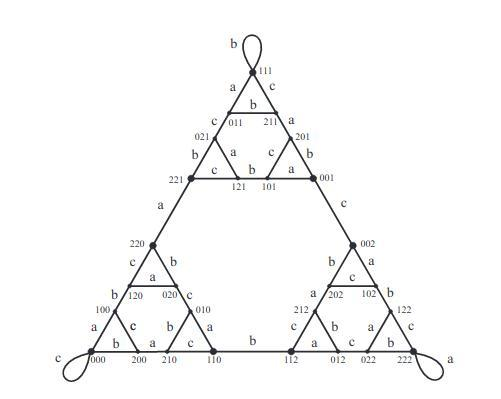
\includegraphics[scale=0.8]{../graphs/SchraierH3.jpg}
	\label{automaton}
	\caption{The Schreier graph of $H^{(3)}$ at level 3.}	
	
\end{figure}

Fix the $n \in \mathbb{N}$ and relative $\Gamma_n$. Consider a finite Mealy automaton 
$A_n = (S_n, S_0, \Sigma, \Lambda, T, G)$, where 

\begin{itemize}
	\item $S_n = \Sigma^n$ - a finite set of states. 
	\item $S_0 = w_n \in S_n$ - a start state
	\item $\Sigma = \{a, b, c\}$ - an input alphabet
	\item $\Lambda = \Sigma$ - an output alphabet 
	\item $T_n: S_n \times \Sigma \rightarrow S_n$ - a transition function 
	\item $G_n: S_n \times \Sigma \rightarrow \Lambda$ - an output function.
\end{itemize}

Define the transition $T_n$ function due to graph $\Gamma_n$ understanding vertices' numbers as words from $\Sigma^n$.
Also define the output function $G_n$ in such a way: 
$$G_n \left( (aaa, a) \right) = a,\quad G_n \left( (bbb, b) \right) = b, \quad G_n \left( (ccc, c) \right) = c$$
and returns empty word otherwise. 

\begin{statement}
	Let $w, v \in H^{(3)}$, $A(v)$ stops in state $S_r$ and returns $v_x$. Then,
	$$ (w v)|_{S_r} = w|_{S_0} v_x.$$
	In other words, automaton $A$ simulates changes of $w_{S_0}$ after multiplying $w$ on $v$.
\end{statement}

\begin{proof}
	Due to properties of multiplication in $H^{(3)}$ multiplying $w$ by $a$ means also multiplying $w|_{a^n}$. Similarly 
	$b$ implies on $w|_{b^n}$ and $c$ on $w|_{b^n}$. Otherwise $w|_x$ does only change its own position (i.e. $x$). Such 
	properties is the conditions the automaton is constructed on.
\end{proof}

\section{Average case. Hypotheses}

Now let's take a look at the aforementioned average size of trees. The main problem is we don't know which level 
is the last because we don't know properties of the tree's height. 

\begin{statement}
	The $k$-th level isn't the last as long as it has at least one element $w_k$ which consists of $\ge 2$ different 
	symbols. 
\end{statement}

As a result for $k$-th level we can investigate how many elements $w \in G, \, |w| = n$ have height $\ge k$ considering 
multiplication $e$ by $w$ as a random walk on the $\Gamma_n$. The path on the $\Gamma_n$ is acceptable for us iff it 
contains at least two different loops. If number of such elements is big enough we can make an estimation for 
asymptotic growth of the average size. 


\newpage

\begin{thebibliography}{9}
	\bibitem{Hanoi1}
	Rostislav Grigorchuk, Zoran Sunik. Asymptotic aspects of Schreier graphs and Hanoi Towers groups. Department of Mathematics, Texas A\&M University, MS-3368, College Station, TX, 77843-3368, USA, 2006
	
	\bibitem{Hanoi2}
	Rostislav Grigorchuk, Zoran Sunik. SCHREIER SPECTRUM OF THE HANOI TOWERS GROUP ON THREE PEGS 2007
	
	\bibitem{Auto}
	R.I. Grigorchuk, V.V. Nekrashevich, V.I. Sushchanskiı, Automata, dynamical systems, and groups, Tr. Mat. Inst. Steklova 231 (2000) 134-214
	(Din. Sist., Avtom. i Beskon. Gruppy).
	
	\bibitem{HRepr}
	Bartholdi, Laurent; Siegenthaler, Olivier; Zalesskii, Pavel. The con-gruence subgroup problem for branch groups,Israel  J.  Math.187(2012),419450.
	
	\bibitem{HaoniDesk} Andreas M. Hinz,The Tower of Hanoi, Enseign. Math. (2)35(1989), 
	no. 3-4, 289–321. MR MR1039949 (91k:05015)
	
\end{thebibliography}

\newpage
\thispagestyle {empty}

\begin{appendices}

\section{Python interface for elements of automaton groups}

A full implementation you can find at \href{https://github.com/davendiy/automata-groups}{github.com/davendiy/automata-groups}

\begin{lstlisting}[language=Python, basicstyle=\tiny]
# File: src/source2.py

class AutomataTreeNode(Tree):
    """ Recursive tree for element of Automata group.
    :param permutation: root permutation of node
    :param value:    name of element (will be printed on picture)
    :param reverse:  True if this node means the recursive callback of
                     the parent (\delta)
    :param simplify: True if it could be drawn as point with name
                     (e.g. for e, a, b, c)
    """
    def __init__(self, permutation=TRIVIAL_PERM, value=None, reverse=False,
                 simplify=False):
        ...
    @property
    def name(self):
        """ Get the name of a node.
        """
        ...

    def height(self) -> int:
        """ Get height of the w's tree. 
        Complexity - \Theta(V) (DFS), where V is amount of vertices.
        """
        ...

    def vert_amount(self) -> int:
        """ Get amount of tree's vertices. 
        Complexity - \Theta(V) (DFS).
        """
        ...

    def size(self) -> int:
        """ Get size w's tree. 
        Complexity - \Theta(V) (DFS).
        """
        ...
	
    def add_child(self, child, position=None):
        """ Add a child (first-level section) to the root of the tree 
        and put it on a (possibly not) given position.

        Complexity - \Theta(W) where W is amount of child's vetices 
        (it adds copy of the child in order to escape cyclics).
        """
        ...
        
    def remove(self, child):
        """ Remove the child (first-level section) of the root.
        Complexity - O(k) where k is amount of root's children.
        """
        ...
	
\end{lstlisting}

\newpage

\begin{lstlisting}[language=python, basicstyle=\tiny]


class AutomataGroupElement:
    """ Implementation of an element of an automaton group.
    
    This class represents any element that has structure 
    g = \pi (g_1, g_2, g_3). Group defines by initialising an alphabet of 
    its generators (a1, a2, a3 ...) using __init__ method and then for every 
    word w from the alphabet corresponding element can be created using 
    function $$$ from_string $$$. 
    
    a = AutomataGroupElement(name, permutation, children)    
    
    :param name: the name of an atom (for instance a, b, c, e for H3)
    :param permutation: object sympy.combinatorics.Permutation
    :param children: a list of AutomataTreeNode or AutomataGroupElement 
                     elements that defines tree-like structure of the 
                     element (first-level state). Those elements 
                     should have $ name $ of the respective atom 
                     or have parameter $ reverse $ with value True 
                     that means recursive call.
     
    Example of using (Hanoi tower group H^3):
    >>> e = AutomataGroupElement('e', simplify=True)
    >>> a = AutomataGroupElement('a', permutation=Permutation([1, 0, 2]), \
                                 children=(e, e, reverse_node()), simplify=True)
    >>> b = AutomataGroupElement('b', permutation=Permutation([2, 1, 0]), \
                                 children=(e, reverse_node(), e), simplify=True)
    >>> c = AutomataGroupElement('c', permutation=Permutation([0, 2, 1]), \
                                 children=(reverse_node(), e, e), simplify=True)
    >>> from_string('abcbabcbabcbabc')
    abcbabcbabcbabc = (0 2) (acacacac, bbb, bbbb)


    As you can see element is completely defined by it's tree structure. 
    The multiplication of two elements is just combining of their trees in 
    some way.
    
    WARNING: you can't create in this way elements that reffers to each other, 
    for example 
                 a = ()(a, b, e)      and  b = ()(b, e, a)
    because such elements don't have tree-like structure. 
    Well in fact, you can do it but I don't guarantee it will work properly.
    """
	
    def __init__(self, name, permutation=TRIVIAL_PERM,
                    children=(AutomataTreeNode(reverse=True),
                              AutomataTreeNode(reverse=True),
                              AutomataTreeNode(reverse=True)),
                    simplify=False):
        ...
	
    def __len__(self):
        """ Returns the |w|. 
        E.g. |e| = 0, |ai| = 1.
        """
        ...
     
    @property
    def permutation(self) -> Permutation:
        ...
        
    def is_trivial(self) -> bool:
        """ Returns whether element is trivial or not (algorithm will be 
        explained a bit later). 
        
        Complexity - O(V), where V is amount of vertices.
        """
        ...
    
    @classmethod
    def from_cache(cls, el: str):
        """ Get already initialised element by name el.
        """
        ...
    
    def __mul__(self, other):
        """ Multiplication of AutomataGroupElements. Complexity - O(V_1 + V_2), 
        where V_1 and V_2 are amount of vertices of self and other respectively.
        """
        ...
    
    def order(self) -> int:
        """ Get the order of the element (algorithm will be explained a bit later).
        """
        ...
    
    # and methods for drawing using matplotlib
    ...
    

def from_string(w: str) -> AutomataGroupElement:
    """ Get element that related to the given string.
    
    For example, you can define atomic elements 'a' 'b' and 'c' and then 
    get an element 'ababababacbcbabc'
    
    Complexity - O(n * V), where n = |w| and V = v(w) (amount of vertices)
    
    :param w: a word over an alphabet formed by atomic elements. 
    """
    ...

def reverse_node():       # auxiliary
    return AutomataTreeNode(reverse=True)
 
    
def initial_state():
    """ Initialise atomic elements for Hanoi tower Group.
    """
    global e, a, b, c
    e = AutomataGroupElement('e', simplify=True)
    a = AutomataGroupElement('a', permutation=Permutation([1, 0, 2]),
                             children=(e, e, reverse_node()), simplify=True)
    b = AutomataGroupElement('b', permutation=Permutation([2, 1, 0]),
                             children=(e, reverse_node(), e), simplify=True)
    c = AutomataGroupElement('c', permutation=Permutation([0, 2, 1]),
                             children=(reverse_node(), e, e), simplify=True)

# initialisation is done during importing of this module
e = a = b = c = ...     # type: AutomataGroupElement
initial_state()

\end{lstlisting}

\end{appendices}


\end{document}
